\documentclass[tikz]{standalone}

\usepackage{tikz}
\usetikzlibrary{arrows,positioning,shapes.geometric}

\begin{document}

% 0
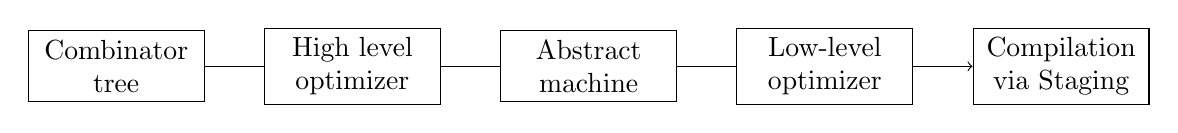
\begin{tikzpicture}%[>=latex']
    \tikzset{block/.style= {draw, rectangle
    , node distance=3cm
    , text width=2cm
    , align=center
      }
    }

\node [block] (init) {Combinator \\tree};
\node [block, right of=init] (node0) {High level optimizer};
\node [block, right of=node0] (node1) {Abstract \\machine};
\node [block, right of=node1] (node2) {Low-level optimizer};
\node [block, right of=node2] (node3) {Compilation via Staging};

 \path[draw, ->]
  (init) -- (node0) -- (node1) -- (node2) -- (node3);
\end{tikzpicture}

\pagebreak

% 1
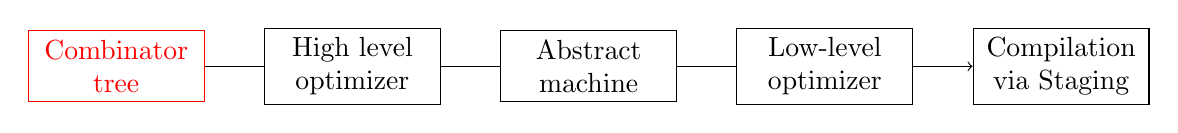
\begin{tikzpicture}
    \tikzset{block/.style= {draw, rectangle
    , node distance=3cm
    , text width=2cm
    , align=center
      }
    }

\node [block,color=red] (init) {Combinator \\tree};
\node [block, right of=init] (node0) {High level optimizer};
\node [block, right of=node0] (node1) {Abstract \\machine};
\node [block, right of=node1] (node2) {Low-level optimizer};
\node [block, right of=node2] (node3) {Compilation via Staging};

 \path[draw, ->]
  (init) -- (node0) -- (node1) -- (node2) -- (node3);
\end{tikzpicture}

\pagebreak
% 2
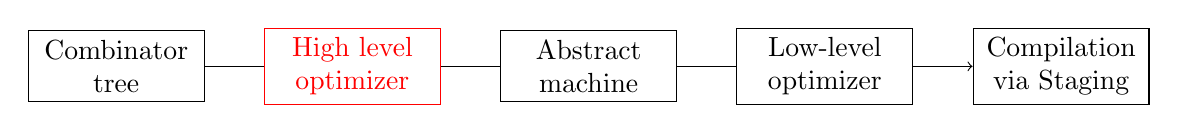
\begin{tikzpicture}
    \tikzset{block/.style= {draw, rectangle
    , node distance=3cm
    , text width=2cm
    , align=center
      }
    }

\node [block] (init) {Combinator \\tree};
\node [block,color=red, right of=init] (node0) {High level optimizer};
\node [block, right of=node0] (node1) {Abstract \\machine};
\node [block, right of=node1] (node2) {Low-level optimizer};
\node [block, right of=node2] (node3) {Compilation via Staging};

 \path[draw, ->]
  (init) -- (node0) -- (node1) -- (node2) -- (node3);
\end{tikzpicture}
\pagebreak

% 3
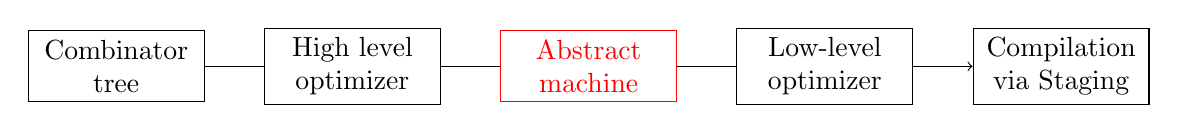
\begin{tikzpicture}%[>=latex']
    \tikzset{block/.style= {draw, rectangle
    , node distance=3cm
    , text width=2cm
    , align=center
      }
    }

\node [block] (init) {Combinator \\tree};
\node [block, right of=init] (node0) {High level optimizer};
\node [block,color=red, right of=node0] (node1) {Abstract \\machine};
\node [block, right of=node1] (node2) {Low-level optimizer};
\node [block, right of=node2] (node3) {Compilation via Staging};

 \path[draw, ->]
  (init) -- (node0) -- (node1) -- (node2) -- (node3);
\end{tikzpicture}

\pagebreak

% 4
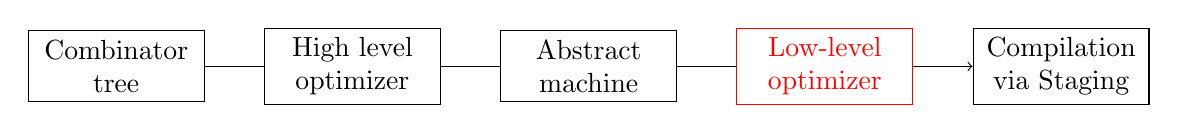
\begin{tikzpicture}
    \tikzset{block/.style= {draw, rectangle
    , node distance=3cm
    , text width=2cm
    , align=center
      }
    }

\node [block] (init) {Combinator \\tree};
\node [block, right of=init] (node0) {High level optimizer};
\node [block, right of=node0] (node1) {Abstract \\machine};
\node [block,color=red, right of=node1] (node2) {Low-level optimizer};
\node [block, right of=node2] (node3) {Compilation via Staging};

 \path[draw, ->]
  (init) -- (node0) -- (node1) -- (node2) -- (node3);
\end{tikzpicture}

\pagebreak

% 5

\begin{tikzpicture}
    \tikzset{block/.style= {draw, rectangle
    , node distance=3cm
    , text width=2cm
    , align=center
      }
    }

\node [block] (init) {Combinator \\Tree};
\node [block, right of=init] (node0) {High level optimizer};
\node [block, right of=node0] (node1) {Abstract \\machine};
\node [block, right of=node1] (node2) {Low-level optimizer};
\node [block,color=red, right of=node2] (node3) {Compilation via Staging};

 \path[draw, ->]
  (init) -- (node0) -- (node1) -- (node2) -- (node3);
\end{tikzpicture}

\pagebreak

\end{document}

\begin{comment}
% https://tex.stackexchange.com/questions/209355/drawing-a-block-diagram-using-tikz/209367

\begin{document}
    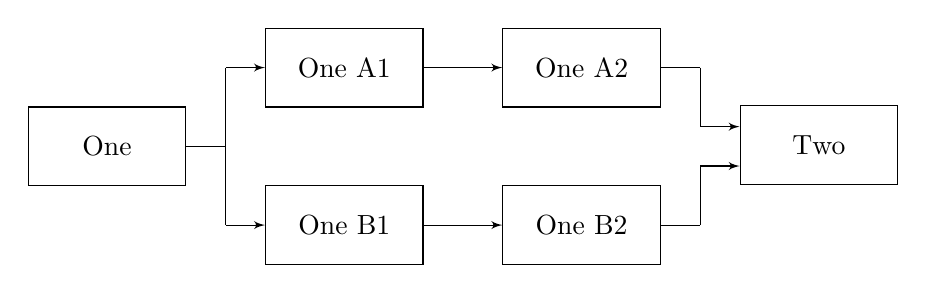
\begin{tikzpicture}[>=latex']
        \tikzset{block/.style= {draw, rectangle, align=center,minimum width=2cm,minimum height=1cm},
        }
        \node [block]  (start) {One};

        \node [coordinate, right = 0.5cm of start] (ADL){};
        \node [coordinate, above = 1cm of ADL] (AUL){};
        \node [coordinate, right = 0.5cm of start] (BUL){};
        \node [coordinate, below = 1cm of BUL] (BDL){};

        \node [block, right = 0.5cm of AUL] (A1){One A1};
        \node [block, right = 0.5cm of BDL] (B1){One B1};

        \node [block, right = 1cm of A1] (A2){One A2};
        \node [block, right = 1cm of B1] (B2){One B2};

        \node [coordinate, right = 0.5cm of A2] (AUR){};
        \node [coordinate, below = 0.75cm of AUR] (ADR){};
        \node [coordinate, right = 0.5cm of B2] (BDR){};
        \node [coordinate, above = 0.75cm of BDR] (BUR){};
        \node [coordinate, right = 0.5cm of BUR] (BEnd){};
        \node [coordinate, right = 0.5cm of ADR] (AEnd){};

        \node [block, above right = 0cm and 1cm of B2] (end){Two};

        \path[draw, ->]
            (start) -- (ADL)
            (ADL) -- (AUL)
            (AUL) edge (A1)
            (A1) edge (A2)
            (A2) -- (AUR)
            (AUR) -- (ADR)
            (ADR) edge (AEnd)

            (start) -- (BUL)
            (BUL) -- (BDL)
            (BDL) edge (B1)
            (B1) edge (B2)
            (B2) -- (BDR)
            (BDR) -- (BUR)
            (BUR) -- (BEnd)
                    ;
    \end{tikzpicture}
\end{document}
\end{comment}